% ------------------------------------------------------------------------
% -*-TeX-*- -*-Hard-*- Smart Wrapping
% ------------------------------------------------------------------------
%%% Literature Survey --------------------------------------------------

%\addtolength{\topmargin}{-.875in}
%\addtolength{\textheight}{.875in}
%\footskip
%\nonumchapter{Literature Survey}
\chapter{Perspectives for Riemannian Approaches}
\label{chap:perspectives-riem} 
\epigraph{Tell me and I forget, teach me and I may remember, involve me and I learn.}{--- \textup{Benjamin Franklin}}
%-------------------------------------------------------------------------

\section{Introduction}%Hybrides, Passive, and Neurofeedback
\label{sec:perspective-intro}

For efficient learning in EEG based BCI, as in most machine learning applications, an important amount of training data is needed. 
However the amount of data available within the BCI community is little \citep{delorme_eeg_2015}. 
Another particularity with BCI is that the inter-subject variability requires that data used for training come from the same subject that the testing ones. 
Because of the difficulties in acquiring long signals from users and the need to keep the calibration time short, such training data are usually not available.
Moreover, in some BCI applications the number of trials per class cannot be determined by the experimental paradigm, resulting in a class imbalance that disturbs the learning process.   

A possible way of solving these problems related to data scarcity is \emph{data augmentation}. 
In this approach, artificial data are generated by applying a transformation to the recorded data \citep{van_dyk_art_2001, grandvalet_anisotropic_2000}.
This technique has been successfully applied on image classification, when the number of samples in each class is small.
The common practice is to identify a set of possible transformations that could affect input images, e.g. rotation, translation, scaling, flipping, brightness adjustment, and to randomly applied those transformations to each training example \citep{dieleman_rotation-invariant_2015}. 
In the context of handwritten character recognition, an elastic distortion emulating uncontrolled oscillation of hand muscles is applied \citep{simard_best_2003}. % \cite{graves2009novel}. 
Figure \ref{fig:mnist-transformations} shows an example of images where translation, scaling, rotation and elastic distortion have been applied. 
\begin{figure}[h!]
\includegraphics[width=1\columnwidth]{Figures/mnist} 
\label{fig:mnist-transformations}
\caption{Hand-written digits from MNIST dataset. The original data are on the first row, the other rows are artificially created images from distorted version of the original digits. \citep[Image taken from ][]{ciresan_multi-column_2012}}
\end{figure} 
Data augmentation works well when combined with artificial neural network \citep{duda_pattern_2001, ciresan_multi-column_2012, krizhevsky_imagenet_2012}.
In BCI applications, a similar approach has been used to reduce calibration time in a motor imagery based BCI system \citep{lotte_generating_2011}.
Each recorded trial is segmented and segments from the original set are randomly selected and concatenated to form new artificial trials. 

In this chapter a novel data augmentation method based on non-Euclidean geometry is proposed. 
Unlike those mentioned above, data are not generated in the input space. 
Each training trial is represented in the space of SPD matrices by its covariance matrix. 
%The space of SPD matrices, with the proper structure and inner product, defines a Riemannian manifold.
The augmented data lives on the manifold and within the convex hull defined by their class set. %of the class to which they belong 
As a result, the convex hull of the class is densified with transformed versions of the original data. 
The augmented data are fed to a classifier, here we consider a multi-layer perceptron. 
This method is evaluated on two experimental datasets.
The first one is an SSVEP-based BCI where only a limited number of training examples are available.
The second one is an error detection application of ERP-based BCI to generate artificial trials to balance the number of positive and negative trials.
In the error related potential (ErrP) application paradigm, the number of trials with and without ErrP variable and not controlled.

Other than data augmentation, another way to make up for missing training data is to use data or parameters learnt from other subjects with sufficient training data. 
This is referred to as \emph{transfer learning}.
Machine learning algorithms aim at learning a task from training data. 
Once a task has been learnt, it can then be applied to future data (also referred to as test data). 
These algorithms work on the assumption that the training data and the future data are drawn from the same feature space and the same distribution.
However, in real life applications, it is not always possible to have training data available, which are drawn from the same feature space and same distribution as the test data. 
Moreover, the task to be performed on new data can differ from the task learned from the training (or previous) data.
Transfer learning thus aims at transferring the knowledge learnt from the previous task and data to a new task and data.


In BCI the need of transfer learning is important due to \textit{inter-subject} variability and \textit{intersession} variability. 
\emph{Inter-subject} variability is expressed by the difference of brain signals recorded from different subjects despite them being involved in the similar mental activities. This difference is mostly attributed to anatomical differences among users. 
BCI algorithms are thus trained on brain signals recorded from a user to be letter used for the same task and on the same user.
\emph{Inter-session} variability is manifest between distinct recording sessions of a unique subject. 
This variability is attributed to changes in the mental states of the user, fatigue, and changes in experimental settings e.g. electrodes placement, environment, stimulations, etc.
To make up for these setbacks, training data should be recorded for every BCI user in a controlled environment and the experimental settings meticulously noted. 
To have enough training data, lengthy recordings are needed, which is not always achievable due to BCI illiteracy, fatigue and discomfort.  
Being able to use data recorded from previous BCI users via transfer learning will \\1) eliminate or shorten the recording of training data, and \\2) improve BCI performance for users with limited training data. 
 
\section{Data Augmentation}
\label{sec:data-aug}

This section presents the proposed approach of augmenting training data examples from their covariance matrices using Riemannian geometry. 
%Firstly, it presents the Riemannian geometry tools and construction of covariance matrices that will be used for data augmentation. 
%Secondly, it presents the proposed method to generate artificial data.
%Thirdly, the results obtained on SSVEP and ERP data are shown. 

%\subsection{Riemannian geometry tools}
% 
%The covariance matrices of SSVEP are obtained from the extended signal \eqref{eq:ext_data} as described in section \ref{sec:mdm}:
%\[
%	\X \in \Re^{\dc \times \dt} \rightarrow 	
%	\begin{bmatrix}
%		X_{\text{freq}_1}\\ \vdots \\ X_{\text{freq}_{\dF}} \\
%	\end{bmatrix}
%	\in \Re^{\dF\dc \times \dt} \ ,
%\]
%
%For ERP paradigm with a number $E$ of different ERPs, the modified signal is the concatenation of the original signal and the grand averages of trials containing the target ERPs $\bar{X}_e$, $e=1, \ldots, E$:
%\begin{equation}
%\X \in \Re^{\dc \times \dt} \rightarrow 	
%\begin{bmatrix}
% \bar{X}_1\\ 
%\vdots \\
%\bar{X}_E \\
%X\\
%\end{bmatrix}
%\in \Re^{(E+1)\dc \times \dt} \ ,
%\label{eq:ext_data_erp}
%\end{equation}
%The resulting covariance matrix will be of size $((E+1) \times \dc)^2$. Adding a non-target class, it is a multiclass classification with $\dK=E+1$ classes.

\subsection{Generating Artificial Points on Riemannian Manifold}
\label{sec:interpolation}

Each trial's covariance matrix being represented as a point on the manifold, artificial trials are generated by interpolating new points between original trials' covariance matrices belonging to one class. 
This interpolation is done on the geodesic connecting each pair of original trials such that the generated point remains on the manifold and within the convex hull of the set of the class original data.
This approach is similar to tensor linear interpolation introduced in \citep{pennec_riemannian_2006}. % \cite{Boissonnat2001}. %Syl: est ce que c'est bien ce papier que tu veux citer ? 
%Emmanuel: J'ai mis celui que je voulais citer.
Given the definition of the tangent vector $\overrightarrow{\P_1 \P_2}$ between $\P_1$ and $\P_2$ in \eqref{eq:tan_geo}, the geodesic $\gamma$ on the manifold can be obtained by the exponential mapping of $\overrightarrow{\P_1 \P_2}$ defined in \eqref{eq:exp_r} as:
$\gamma = \Exp{\P_1}(\Log{\P_1}(\P_2))$. 
Defining $t \in [0;1]$, points lying on the geodesic are defined by:
\begin{equation}
\label{eq:inter}
\begin{split}
\P(t) & = \Exp{\P_1}(t ~ \Log{\P_1}(\P_2))\\ 
& = \P_1^{\frac{1}{2}} ( \P_1^{-\frac{1}{2}} \P_2 \P_1^{-\frac{1}{2}} )^t \P_1^{\frac{1}{2}}  
\end{split}
\end{equation} 
with $\P_1 = \P(0)$ and $\P_2 = \P(1)$. Remark that the interpolation \eqref{eq:inter} is equivalent to $(1-t)\P_1 + t\P_2$ in Euclidean space.
Artificial points for data augmentation are obtained between original points by setting $t$ in \eqref{eq:inter} to any value other than $0$ and $1$.
In our experiments, interpolated matrices between each pair $\P_1,\P_2$ are linearly spaced on the geodesic between $0$ and $1$, and all possible pairs are considered.

Outliers in the pool of original data covariance matrices can distort the convex hull of classes, resulting in misclassification of new trials.
To alleviate these effects, outliers are rejected from the original data before the generation of artificial data using an offline Riemannian potato described in section \ref{sec:potato}. 
The Riemannian mean of matrices belonging to one class is used as the centre of the Riemannian potato for that class. 
% \textcolor{blue}{Quentin: question, une patate par classe? si oui, mieux préciser}
% \textcolor{blue}{Emmanuel: Oui c'est une patate par classe. C'est claire comme ca?}
% \textcolor{blue}{Quentin: ok pour moi!}
For each class, all matrices beyond the z-score of 1 from the class centre are rejected.
This value has been chosen after careful cross-validation. 
% \textcolor{blue}{Quentin: mais preciser comment la valeur atypique de 1 est choisie.}

\subsection{Classification}

To evaluate the benefit of applying the proposed data augmentation method, three classifiers are considered: a multi-layer perceptron (MLP) neural network \citep{duda_pattern_2001} which is used on original data and then on augmented data, a tangent space linear discriminant analysis (TSLDA) \citep{barachant_multiclass_2012} and a Riemannian-kernel support vector machine (RK-SVM) \citep{yger_review_2013}. 
%The classifiers are trained with the small sets of original data and then with larger sets of augmented data. 
%\textcolor{red}{I can explain the choice of MLP here or in the discussion of results. The details of the MLP in results (because the architecture depends on the number of examples which is only mentioned later)}.
The choice for a MLP is motivated by the fact that neural networks are known to be sensitive to the amount and diversity of examples of data they are presented with \citep{ciresan_multi-column_2012,krizhevsky_imagenet_2012}. 
On the other hand, RK-SVM and TSLDA are versions of SVM and LDA adapted to data lying on a Riemannian space. They are arguably the state-of-the-art concerning EEG covariance classification in tangent space \citep{barachant_multiclass_2012,barachant_classification_2013}.
% \textcolor{blue}{Quentin: heu... le RK-SVM est appliqu\'e dans le plan tangent si je ne m'abuse... En fait, ces deux m\'ethodes travaillent dans le plan tangent.}  
% \textcolor{blue}{Emmanuel: Bon. oui. Maintenant oui. Avant j'essayai de passer une kernel matrix calcul\'ee \`a base de la distance riemannienne \`a une SVM. Donc ce n'etait pas sur le plan tangent. Mais il y a encore quelques discussions \`a faire \`a ce propos. Donc je l'ai retir\'e et pass\'e tout sur la plan tangent. Je viens donc de changer aussi le text ci-dessus} 
% \textcolor{blue}{Quentin: ok}
The classification features $w \in \mathbb{R}^{C(C+1)/2}$ are obtained projecting matrices on the tangent space at their mean $\bar{\P}$:
\begin{equation}
	\label{eq:features}
	\S_i = \bar{\P}^{-\frac{1}{2}} \Log{\bar{\P}}(\P_i) \bar{\P}^{-\frac{1}{2}} = \Logm(\bar{\P}^{-\frac{1}{2}}\P_i \bar{\P}^{-\frac{1}{2}}) \ ,
\end{equation}
and then extracting the upper triangular part of a symmetric matrix $\S_i$ and vectorising it (applying $\sqrt {2}$ weight for out-of-diagonal elements).
These 3 classification methods are offline since the feature extraction \eqref{eq:features} requires the projection on the global mean. However, online extensions are possible \citep{barachant_classification_2013,kalunga_using_2015}.

%****************************************************************************************
\subsection{Experimental Data Description}
\label{sec:data}

The assessment of the proposed data augmentation method is conducted on two datasets.
The first one is from the SSVEP-based experiment described in section \ref{subsec:material-recording}.
The second dataset is an error-related potential detection, where the number of positive examples (the error potential) is smaller than the number of negative examples, that is a problem with unbalanced classes.
Here only the ERP dataset is described.

\subsubsection{ERP Dataset}
The dataset, available for the NER Kaggle competition, was recorded during an online P300 speller experiment for error detection in the speller \cite{margaux_objective_2012}.
16 healthy subjects participated in the experiment, the brain activity was recorded on $\dc=56$ channels. 
%A 6 x 6 matrix of flashing items is used for stimulation. 
%The stimuli are flashed in a pseudo random order. 
%When the item (i.e. letter) on which the subject is focusing is attention is flashed, a positive deflection (i.e. P300) in the EEG occurs approximately 300 ms later. 
%The selected item is identified by detecting a P300 after it has been flashed. 
Subjects have to spell a series a letter in under two spelling conditions: a fast, more error-prone condition (each item is flashed 4 times), and a slower, less error-prone (each item is flashed 8 times). 
The subjects had to go through five spelling sessions. 
Each session consisted of twelve 5-letter words, except the fifth which consisted of twenty 5-letter words making up for a total of 340 letters. 
For each spelled letter, the feedback of the result of the speller is displayed on a screen.
The time of feedback is recorded and the label of feedback (correct or incorrect) is also recorded. 
In case of a spelling error, an error evoked potential occurs in the EEG. 
In the current work we focus on the detection of the error in spelling based on this \emph{a priori}. 
The task of learning algorithms is to detect errors, \textit{i.e.} to classify trials as incorrect or correct ($K=2$, positive or negative). 
In such experiments, the number of positive and negative trials is not balanced. 
In case of a good speller, the number of positive trials are very limited. 
In this dataset the number of positive trials is largely inferior to the number of negative trials creating a problem of class unbalance in training set.
To balance training set from this experiment, artificial data can be generated in the class with less number of trials.

%%%%%%%%%%%%%%%%%%%%%%%%%%%%%%%%%%%%%%%%%%%%%%%%%%%%%%%%%%%%%%%

\subsection{Results and Discussion}
\label{sec:results}
%The efficiency of the proposed approach of generating artificial data is evaluated with an artificial neural network, a Multi-Layer Perceptron (MLP).

\subsubsection{SSVEP dataset}
SSVEP training set is augmented with different numbers of artificial samples for each class. 
%Data are augmented per class. 
One to five samples are interpolated between each pair of original samples belonging to a single class.
Figure~\ref{fig:original-augmented} shows the densification effect resulting from the augmentation process. 
Original covariance matrices of each class are projected on the tangent space computed at the mean of all the matrices, and the two principal components (obtained by applying PCA) are shown on Fig.~\ref{fig:original-class}.
Similarly, Fig.~\ref{fig:augmented-class} shows the augmented covariance matrices after interpolation of 5 points between each pair of covariance matrices within each class. The augmented data are within the convex hull of the original data. 

% \textcolor{blue}{Quentin. petite subtilit\'e a noter : le passage dans le plan tangent, ce n'est pas \eqref{eq:log_r}, mais \eqref{eq:features}!}

\begin{figure}[ht!]
\begin{adjustbox}{center}
\resizebox{1.2\textwidth}{!}{
\subfigure[]{
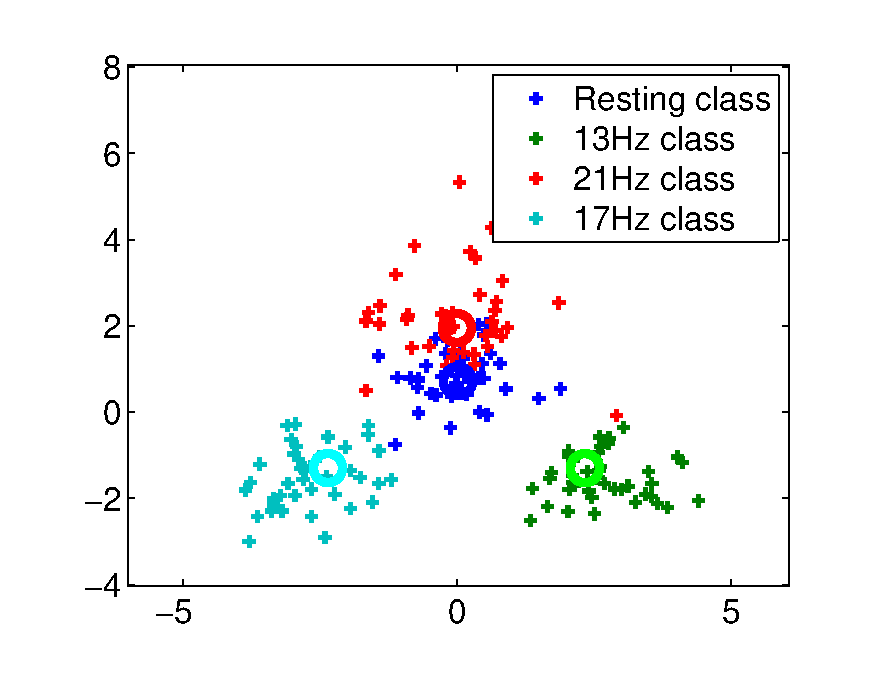
\includegraphics[width=0.8\columnwidth]{Figures/original_class.eps}
\label{fig:original-class}
}
\subfigure[]{
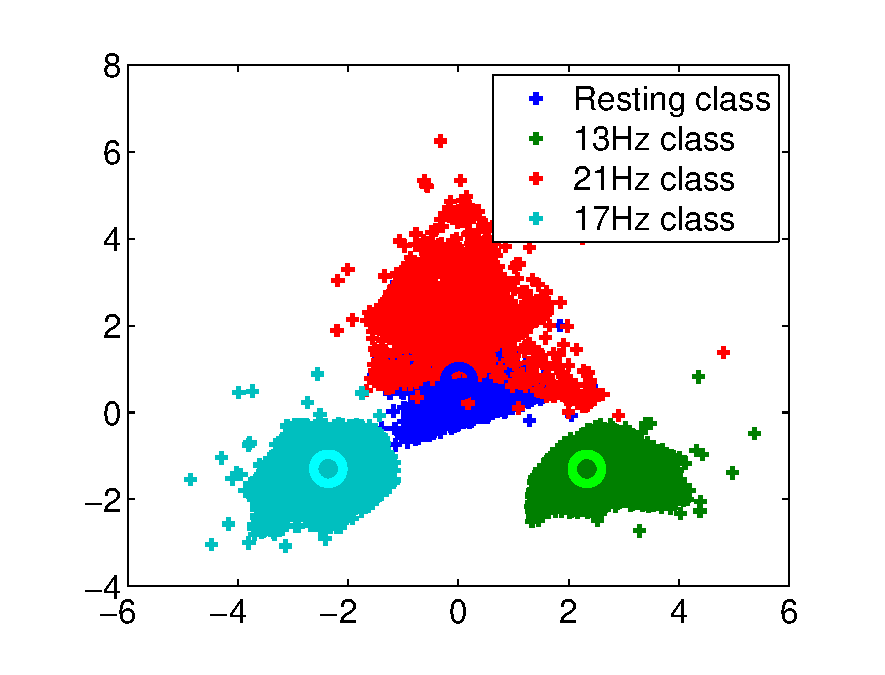
\includegraphics[width=0.8\columnwidth]{Figures/augmented_class.eps}
\label{fig:augmented-class}
}
}
\end{adjustbox}
\caption{Mapping of covariance matrices of trials from each class on the tangent space \eqref{eq:log_r}. Matrices on the tangent space are vectorised and the 2 most significant components from PCA are used to obtain the 2-D representation. The covariance matrices of original data (a) and augmented data (b).} % original + artificial covariance matrices.} 
\label{fig:original-augmented}
\end{figure}

The performance of the augmentation approach is evaluated in terms of classification accuracy obtained with an MLP classifier and the results are compared with those obtained with TSLDA and RK-SVM classifiers. 
The MLP inputs are trial covariance matrices mapped on the tangent space. 
The MLP has 108 input units, one hidden layer with 50 neurons, and 4 output units.
The classification obtained with each number of interpolated points are compared to the performance without training set augmentation. 
Figure~\ref{fig:ssvep-mean} shows the classification performances from zero interpolated point (no training set augmentation) to 5 points interpolated. Due to the non-convexity of MLP optimisation, results averaged over subjects, are then averaged over 10 repetitions.
Significant p-values show that average classification across all subjects is improved by the data augmentation. % when the  by augmenting the training set. 
The effect of data augmentation varies depending on the quality of training examples from individual subjects. 
In Figure~\ref{fig:lowest-highest}, the effect of augmenting training data in the subject with the lowest BCI performance and the subject with highest BCI performances are put side by side. 
%The accuracy improvement in the subject with lowest BCI performance is significant, which is not the case for the subject with highest performance. 
In Table~\ref{tab:res_ssvep}, the classification accuracy (in \%) of the MLP preceded with data augmentation are compared with RK-SVM and TSLDA.
%\textcolor{blue}{Quentin: cette Table~\ref{tab:res_ssvep} est a jour avec les derniers resultats?} 

\begin{figure}[ht!]
\vskip 0.2in
\begin{center}
\centerline{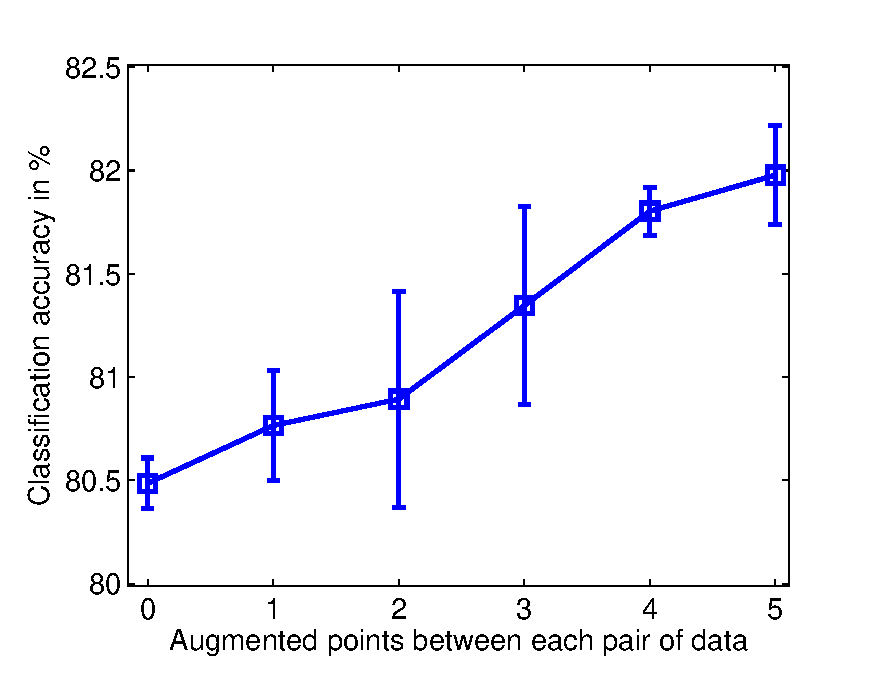
\includegraphics[width=0.95\columnwidth]{Figures/ssvep_mean.eps}}
\caption{Mean classification accuracy in \% across all subjects for different levels of data augmentation. At 0, there is no augmented data. At 1, one artificial data is interpolated between each pair of original data within each class, and so forth}
\label{fig:ssvep-mean}
\end{center}
\vskip -0.2in
\end{figure} 

\begin{figure}[ht!]
\vskip 0.2in
\begin{center}
\centerline{\includegraphics[width=0.95\columnwidth]{Figures/subjects_lowest_highest.eps}}
\caption{Classification accuracy of subject with lowest BCI performance versus subject with highest BCI performance, using original training set and using augmented training set with 5 interpolated points between each pair of original data within each class.}
\label{fig:lowest-highest}
\end{center}
\vskip -0.2in
\end{figure} 

    
\begin{table}[ht!]
\centering
\ra{1}
\begin{tabular}{c|c|c|c|c|}
\cline{2-5}
&  MLP & aug+MLP & RK-SVM & TSLDA \\ \cline{1-5}

\multicolumn{1}{ |c| }{Sub 1}  & 70.63 &  70.63 &  68.75 &  \textbf{73.44} \\ \hline
\multicolumn{1}{ |c| }{Sub 2}  & 71.25 &  78.28 &  \textbf{82.81} &  76.56 \\ \hline
\multicolumn{1}{ |c| }{Sub 3}  & 94.22 &  \textbf{95.00} &  93.75 &  93.75 \\ \hline
\multicolumn{1}{ |c| }{Sub 4}  & 84.06 &  86.72 &  92.19 &  \textbf{93.75} \\ \hline
\multicolumn{1}{ |c| }{Sub 5} & \textbf{73.75} &  67.50 &  \textbf{73.44} &  71.88 \\ \hline
\multicolumn{1}{ |c| }{Sub 6}  & 84.84 &  \textbf{87.66} &  82.81 &  84.38 \\ \hline
\multicolumn{1}{ |c| }{Sub 7}  & 90.73 &  \textbf{91.67} &  89.58 &  90.63 \\ \hline
\multicolumn{1}{ |c| }{Sub 8}  & 89.22 &  \textbf{92.19} &  89.06 &  90.63 \\ \hline
\multicolumn{1}{ |c| }{Sub 9}  & \textbf{70.78} &  68.28 &  62.50 &  67.19 \\ \hline
\multicolumn{1}{ |c| }{Sub 10}  & 78.44 &  76.72 &  \textbf{78.91} &  78.13 \\ \hline
\multicolumn{1}{ |c| }{Sub 11}  & 63.28 &  \textbf{72.97} &  71.88 &  70.31 \\ \hline
\multicolumn{1}{ |c| }{Sub 12}  & 94.62 &  \textbf{96.13} &  \textbf{95.63} &  93.13 \\ \hline \hline
\multicolumn{1}{ |c| }{Average}  & 80.49 &  \textbf{81.98} &  81.78 &  \textbf{81.98} \\ \hline
\end{tabular} 
\caption{Comparison of classification accuracy (in \%) using the MLP on original dataset, MLP with data augmentation (aug+MLP), RK-SVM and TSLDA.}
\label{tab:res_ssvep}
\end{table}

\subsubsection{ERP Dataset}

On the ERP dataset the data augmentation is done to balance the number of positive trials (incorrect P300 feedback where ErrP is present) and negative trials (feedback with no error) in the training set.
Each subject has 240 or 280 trials in the training set. The number of positive trials can be as low as 2\% of the training set. %syl: quel est le nombre de point dans chaque classe, au moins pour donner une idée du déséquilibre entre les classe.
The number of generated artificial trials $g$ is determined by the gap between the number of positive trials and negative trials in the training set. 
To generate $g$ trials, a covariance matrix is interpolated between $g$ pairs of randomly selected original matrices.
The effect of balancing classes with artificial trials is evaluated with the three classifiers (\textit{i.e.} MLP, TSLDA and RK-SVM).
The MLP has 10 input units, one hidden layer with 50 neurons and two output units. 
The number of MLP units is chosen after a cross-validation phase.

% \textcolor{blue}{Quentin: les deux phrases precedentes sont a remonter et fusionner avec la partie methodo.} 
% \textcolor{blue}{Emmanuel: Dans la partie methodo, j'ai pas mis de details experimentaux, du coup je peense que ces deux phrase ne vont pas beaucoup coller l\`a bas. J'ai le meme type d'info pour la SSVEP ici.}
% \textcolor{blue}{Quentin: oui, tu as raison. le nb exact de neurones est a mettre dans la partie experimentale. par contre, il faut expliquer en partie méthodo comment nous sommes arrives à l'architecture actuelle: 1 couche et 50 neurones. cross-validation?}
Since the class unbalance is still present in the evaluation set, the classification performances are evaluated in terms of sensitivity.
Figure~\ref{fig:sensitivity-auc} shows the performance achieved when classes are balanced by augmenting data in the positive class. 
They are compared to the results achieved when using unbalanced training set. A t-test was performed and the p-values reveal significant improvement after data augmentation. Table \ref{tab:res-sensitivity} shows details of classifiers performance per subject in terms of sensitivity with and without data augmentation.   

\begin{figure}[ht!]
\centering
% \subfigure[]{
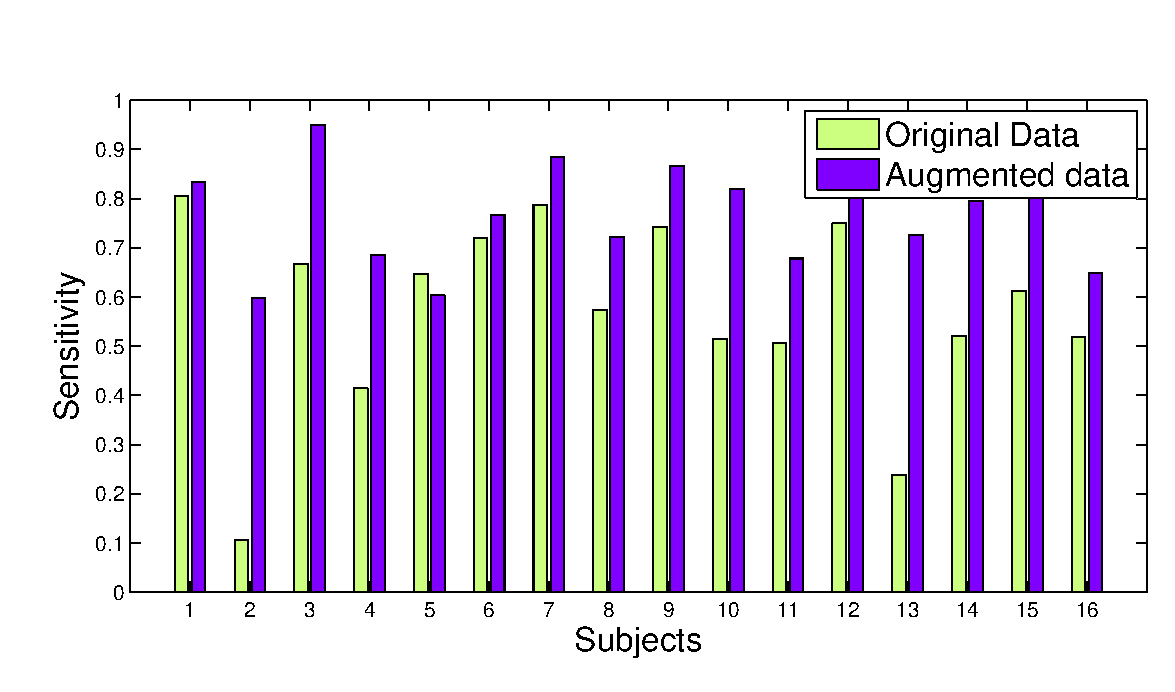
\includegraphics[width=1\columnwidth]{Figures/erp_sensitivity.eps}	
\label{fig:erp-sensitivity}
% }
% \subfigure[]{
% \includegraphics[width=0.8\columnwidth]{Figures/erp_auc.eps}
% \label{fig:erp-auc}
% }
\caption{Classification performance in terms of %(a) 
sensitivity. % and (b) AUC. 
For each of the 16 subjects these measures are given for classification based on training on original unbalance training set and training on augmented and balanced training set. 
%The p-values indicating the significance of improvement brought by data augmentation for each subject is shown with a star on the subject sensitivity bars: significant improvements are denoted by red/thick stars, and non-significant ones by blue/thin stars (null hypothesis rejected at the 5\% significance)
} 
\label{fig:sensitivity-auc}
\end{figure} 


\begin{table*}[ht!]
\centering
\ra{1}
\begin{tabular}{c|c|c|c||c|c|c|}
\cline{2-7}
&  \multicolumn{3}{ c||}{Imbalanced classes} & \multicolumn{3}{ c| }{Balanced classes} \\ \cline{1-7}
\multicolumn{1}{ |c| }{Sub.} & MLP & RK-SVM & TSLDA & MLP & RK-SVM & TSLDA \\ \hline
\multicolumn{1}{ |c| }{1}   & 0.85  &  0.76  &  0.79  &  0.83  &  0.77  &  \textbf{0.85} \\ \hline
\multicolumn{1}{ |c| }{2}   & 0.11  &   0  &  0.32  &  \textbf{0.60}  &  0.07  &  0.57 \\ \hline
\multicolumn{1}{ |c| }{3}   & 0.67  &  0.60  &  0.72  &  \textbf{0.95}  &  0.63  &  \textbf{0.95} \\ \hline
\multicolumn{1}{ |c| }{4}   & 0.41  &  0.42  &  0.63  &  0.69  &  0.32  &  \textbf{0.70} \\ \hline
\multicolumn{1}{ |c| }{5}   & 0.65  &  0.51  &  0.61  &  0.60  &  0.49  &  \textbf{0.68} \\ \hline
\multicolumn{1}{ |c| }{6}   & 0.72  &  0.71  &  0.74  &  \textbf{0.77}  &  0.70  &  0.76 \\ \hline
\multicolumn{1}{ |c| }{7}   & 0.79  &  0.70  &  0.78  &  0.88  &  0.70  &  \textbf{0.89} \\ \hline
\multicolumn{1}{ |c| }{8}   & 0.57  &  0.33  &  0.63  &  \textbf{0.72}  &  0.25  &  0.70 \\ \hline
\multicolumn{1}{ |c| }{9}   & 0.74  &  0.59  &  0.77  &  0.87  &  0.58  &  \textbf{0.89} \\ \hline
\multicolumn{1}{ |c| }{10}   & 0.51  &  0.34  &  0.59  &  0.82  &  0.34  &  \textbf{0.90} \\ \hline
\multicolumn{1}{ |c| }{11}   & 0.51  &  0.27  &  0.57  &  \textbf{0.68}  &  0.27  &  0.61 \\ \hline
\multicolumn{1}{ |c| }{12}   & 0.75  &  0.65  &  0.82  &  0.97  &  0.65  &  \textbf{0.99} \\ \hline
\multicolumn{1}{ |c| }{13}   & 0.24  &     0  &  0.57  &  0.73  &  0.08  &  \textbf{0.75} \\ \hline
\multicolumn{1}{ |c| }{14}   & 0.52  &  0.47  &  0.62  &  \textbf{0.80}  &  0.43  &  0.75 \\ \hline
\multicolumn{1}{ |c| }{15}   & 0.61  &  0.51  &  0.65  &  0.81  &  0.60  &  \textbf{0.83} \\ \hline
\multicolumn{1}{ |c| }{16}   & 0.52  &  0.46  &  0.54  &  \textbf{0.65}  &  0.42  &  0.53 \\ \hline \hline
\multicolumn{1}{ |c| }{Average}   & 0.570  &  0.459  &  0.648  &  \textbf{0.773}  &  0.46  &  0.772 \\ \hline
\end{tabular}
\caption{Sensitivity analysis of performances obtained with 3 classifiers trained with imbalanced training set versus trained with balanced training set. The class imbalance of the ERP dataset is solved with data augmentation.}
\label{tab:res-sensitivity}
\end{table*}

% \textcolor{blue}{Quentin: des AUROC egale a 0? es-tu sur de ton calcul? si c est pas le cas, autant garder ça pour plus tard... La qualit\'e du papier est bien suffisante pour un simple Workshop.} 

% Balancing classes increases the sensitivity to error trials. %However the AUC is slightly reduced for the majority of the subjects.  

%%%%%%%%%%%%%%%%%%%%%%%%%%%%%%%%%%%%%%%%%%%%%%%%%%%%%%%%%%%%%%%

%\subsection{Conclusion}
%\label{sec:conclusion}
%
%In BCI, datasets with reduced numbers of samples and unbalanced classes are frequent.
%This contribution introduces a data augmentation scheme based on the geometry of covariance matrices.
%From the geodesics passing through pairs of samples, new samples are drawn and fed to a neural classifier. 
%The data augmentation allows to boost the classification accuracy when there is only a few number of samples per class.
%It is also possible to compensate for dataset with unbalanced classes as it is often the case in event-related potential paradigm.
%The choice of the classifier is important when dealing with this augmented data; neural networks yields the best results.
%Future works will focus on the optimization of the neural networks: determining the best architecture (in term of layers and neurons) for processing covariance matrices and the investigation of common deep learning methods to improve results (dropouts, ReLU units, etc). 
 
\section{Transfer Learning}
\label{sec:transfer-learn}

\subsection{User Specificity as Domain in Transfer Learning}
\label{subsec:transfer-learning-definition}
%User specificity seen as different domain. Changer le debut du Paragraph

Exposed to the same stimuli, BCI users do not produce similar EEG response. To users specificities should be added changes induced by different environmental conditions during recording. 
In this work, we consider this specificity of the recorded EEG as being different domains in transfer learning. 

\begin{defn}(\emph{Transfer Learning})
\label{def:def1}
Given a source domain $\Dtr_S$ and learning task $\Ttr_S$, a target domain $\Dtr_T$ and learning task $\Ttr_T$, transfer learning aims at improving the learning of the target predictive function $\ftr_T(\cdot)$ in $\Dtr_T$ using the knowledge in $\Dtr_S$ and $Ttr_S$, where $\Dtr_S \neq \Dtr_T$, or $\Ttr_S \neq \Ttr_T$ \citep{pan_survey_2010}.
\end{defn}

Considering the above definition of transfer learning, a domain is a pair $\Dtr = \{\Xtr, P(X)\}$ consisting of a feature space $\X$ and a marginal probability distribution $P(X)$, where $X = \{x_1, \dots, x_n\} \in \Xtr$. 
A task is defined as a pair $\Ttr = \{\Ytr,\ftr(\cdot)\}$ consisting of a label space $\Ytr$ and an objective predictive function $\ftr(\cdot)$ that can be learned from the training data, which consist of pairs $\{x_i, y_i\}$, where $x_i \in X$ and $y_i \in \Ytr$. From a probabilistic viewpoint, $\ftr(x)$ can be written as $P(y|x)$. Thus a task can be defined as $\Ttr = \{\Ytr,P(Y|X)\}$. 
 
\subsection{Category of Proposed Transfer Learning} 
\label{subsec:transfer-learning-category}

In definition~\ref{def:def1}, $\Dtr_S \neq \Dtr_T$, implies that either $\Xtr_S \neq \Xtr_T$ or $P(X_S) \neq P(X_T)$; and $\Ttr_S \neq \Ttr_T$ implies that either $\Ytr_S \neq \Ytr_T$ or $P(Y_S|X_S) \neq P(Y_T|X_T)$.
Depending on each case, the following categories of transfer learning are defined \citep{pan_survey_2010}: 
\begin{enumerate}
\item $\Ttr_S = \Ttr_T$ and $\Dtr_S = \Dtr_T$: Traditional Machine Learning (no transfer)
\item $\Ttr_S \neq \Ttr_T$: \emph{Inductive transfer learning} and \emph{Unsupervised transfer learning}
\item $\Dtr_S \neq \Dtr_T$: \emph{Transductive transfer learning}  
\end{enumerate}

In BCI classification task, both inductive transfer learning and transductive transfer learning can be applied.
In transductive learning, no labelled data are needed from the target domain, while few or all unlabelled data are needed at training time in order to obtain the marginal probability for the target data. 
This situation is suitable in offline BCI applications, and completely eliminate the need for training data, i.e. no recording phase.

In inductive learning few labelled data from the target data are needed to induce the predictive function. 
In this case just a small training set is needed shortening the recording of training data. 
This type of transfer can be used in both offline and online applications.  

%Depending on what is being transfer from the source domain to the target domain, another taxonomy of transfer learning is defined:
%
%\begin{itemize}
%\item
%\end{itemize}

In this work, we are interested in a transductive  transfer learning. 

\subsection{Composite Riemanian Mean}
\label{subsec:composite-riem-mean}

Composite Riemanian Mean is an \emph{instance transfer} technique, \textit{i.e.} re-weighting of labelled data in source domain for use in the target domain \citep{pan_survey_2010}, inspired from the composite common spatial patterns method proposed by \citep{kang_composite_2009} as a feature representation transfer technique.
Data from subjects in source domain are weighted based on the subject's similarity to the subject in the target domain. 
The measure of subjects' similarity is based on the Kullback–Leibler divergence (KL-divergence) as proposed by \citep{kang_composite_2009}. 
Additionally the Affine Invariant Riemannian metric (AIRM) is also used for analysis. Other distances and divergences introduced in Section \ref{subsec:mean} might be used. 
These weights are obtained in an unsupervised way; no labels are required nor in the target domain, nor in the source domain.
We rewrite the definition of the KL-divergence of multivariate Gaussian distribution $\X_1$ and $\X_2$, with covariance matrices $\P_1$ and $\P_2$ respectively from \eqref{eq:div-kl} as:
\[
\divB{KL}(\X_1,\X_2) = \frac{1}{2} \left( \log \frac{\det \P_2}{\det \P_1} - \dc + \text{tr}(\P_2^{-1} \P_1) + (\mu_2-\mu_1)^T \P_2^{-1}(\mu_2-\mu_1) \right)
\]
In the preprocessing, the DC component of EEG signals is removed: $\X \in N(0,\P)$; and the covariance matrices are det-normalized.
Therefore the KL-divergence can be expressed by:
\[
\divB{KL}(\X_1,\X_2) = \frac{1}{2} \left( \text{tr}(\P_2^{-1} \P_1 - \dc)  \right)
\]
Where $\dc$ is the dimension of $\P$, and $\text{tr}(\cdot)$ denotes the trace of a matrix.\\
In Section \ref{sec:bregman-divergence}, a symmetrised version of the KL-divergence was presented as the Jeffreys divergence. It can be expressed as:
\begin{equation}
\divB{KL}^s(\X_1,\X_2) = \sqrt{  \frac{1}{2} \left( \text{tr}(\P_2^{-1} \P_1 + \P_2 \P_1^{-1} - 2 \eye_{\dc})  \right)  } 
\label{eq:KLDs}
\end{equation}
Where $\eye_{\dc}$ is the identity matrix of size $\dc$.
 
The AIRM ($\distAIRM(\P_1, \P_2)$) is defined by \eqref{eq:dist_air}

The similarity between two subjects is defined as the inverse of the KL-divergence of their recorded EEG signals (or AIRM of their covariance matrix):
\begin{equation}
\simil_{j,k} = \frac{1}{Z^k} \cdot \frac{1}{\divB{KL}(\X_j, \X_k)}
\label{eq:sim}
\end{equation}
Where $Z^k$ is a normalisation factor for all distances to subject k:
\begin{equation}
Z^k = \sum_{l \neq k} \frac{1}{\divB{KL}(\X_l,\X_k)}
\label{eq:normk}
\end{equation} 
For the AIRM, $\divB{KL}(\cdot,\cdot)$ is replaced by $\distAIRM(\cdot, \cdot)$ in Equations~\eqref{eq:sim} and \eqref{eq:normk}.

To classify samples from the target subject $k$ using MDRM, \emph{composite Riemannian means} of classes are obtained as:

\begin{equation}
\ccm^k = (1-\lambda)\cm^k + \lambda \sum_{j \neq k} \simil_{j,k} \cm^j
\label{eq:ccm}
\end{equation}
where $\cm$ is the individual subject's mean of class $c$, and $\lambda \in [0,1]$.

\subsubsection{Defining parameter $\lambda$}

In \eqref{eq:ccm}, the parameter $\lambda$ defines how much the classification relies on data from other subjects. 
When a subject has enough and clean training data, it might not be necessary to use data from other subject; when the subject has noisy or little data, or his or her training data cannot be trusted, it might be safer to rely more on data from other subjects. The balance between this cases is determined by $\lambda$.
We identified that $\lambda$ will depend mainly on the number of data available for the test subject, and the proximity (or similarity) of this subject to other subjects. In other words, the proximity is also a measure of data transferability. 
We define $\lambda$ as a flipped logistic function of the similarity of the test subject to other subjects and the number of training samples available per class in the training data of the test subject:
\begin{equation}
\lambda = \frac{1}{1+e^{az(n-n_0)}}
\label{eq:lambda}
\end{equation}
\begin{description}
\item[$a$]: $a \geq 1$, parameters controlling the decay. It can be learnt through cross-validation process.
\item[$z$]: Normalised z-score used as proximity measure. 
\item[$n$]: Number of labelled samples per class.
\item[$n_0$]: $n_0 > 1$ Shift in logistic function. It can be learnt through cross-validation process.
\end{description}

\subsection{Experimental Results}

\subsubsection{Subjects similarity and weighting}
\begin{figure}[h!]
\centering
\subfigure[]{
\includegraphics[width=0.47\textwidth]{Figures/subjects_similarity_AIR.eps}
\label{fig:subjects_similarity_AIR}}
\subfigure[]{
\includegraphics[width=0.47\textwidth]{Figures/subjects_similarity_KL_up.eps}
\label{fig:subjects_similarity_KL_up}}
\subfigure[]{
\includegraphics[width=0.47\textwidth]{Figures/subjects_similarity_KL_low.eps}
\label{fig:subjects_similarity_KL_low}}
\subfigure[]{
\includegraphics[width=0.47\textwidth]{Figures/subjects_similarity_KL_bar.eps}
\label{fig:subjects_similarity_KL_bar}}

\caption{2-D representation of affinity (or similarity) between subjects based on the 4 metrics: \ref{fig:subjects_similarity_AIR}: Affine Invariant Riemannian distance, \ref{fig:subjects_similarity_KL_up}: Kullback-Leibler using forward divergences, \ref{fig:subjects_similarity_KL_low}: Kullback-Leibler using reverse divergences, \ref{fig:subjects_similarity_KL_bar}: the symmetric version of KL divergence.}
\end{figure}

\subsubsection{Grid search}

A grid search is performed for $\lambda \in \left\lbrace 0, 0.2, 0.4, 0.6, 0.8, 1 \right\rbrace$.
The number of labelled training examples from the test subject -- used in the computation of $\cm^k$ in Eq.~\eqref{eq:ccm}, is also varied: $n \in \left\lbrace 4, 8, 12, 16, 20, 24, 28, 32 \right\rbrace $.  

\begin{figure}[h!]
\centering
\subfigure[]{
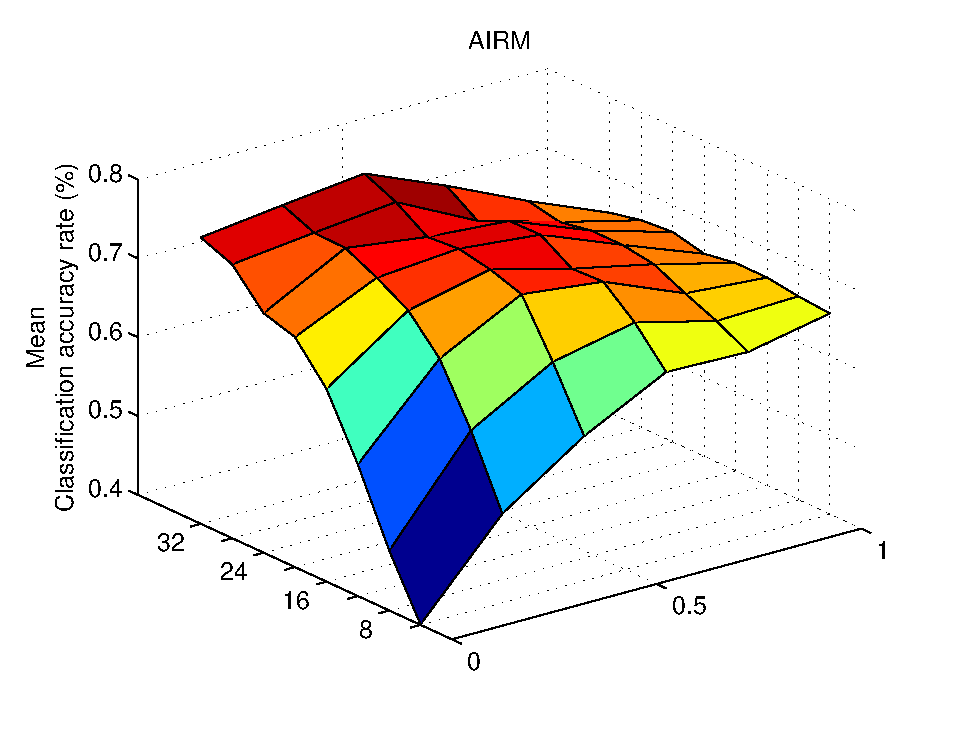
\includegraphics[width=0.47\textwidth]{Figures/surfmean_airm.eps}
\label{fig:surfmean_airm}}
\subfigure[]{
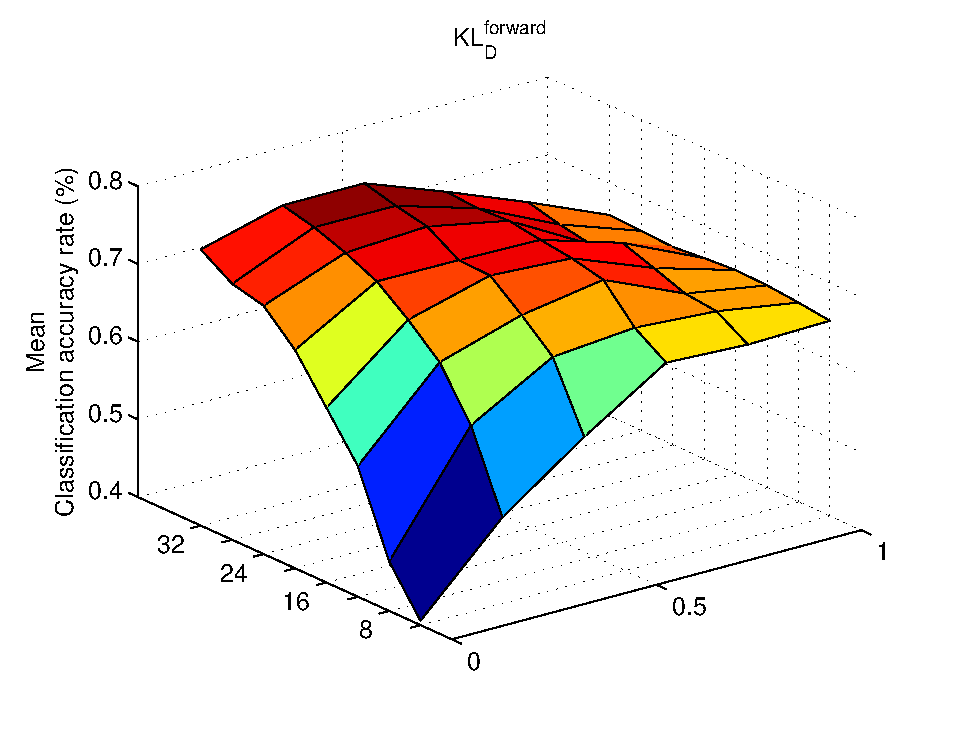
\includegraphics[width=0.47\textwidth]{Figures/surfmean_kld_for.eps}
\label{fig:surfmean_kld_for}}
\subfigure[]{
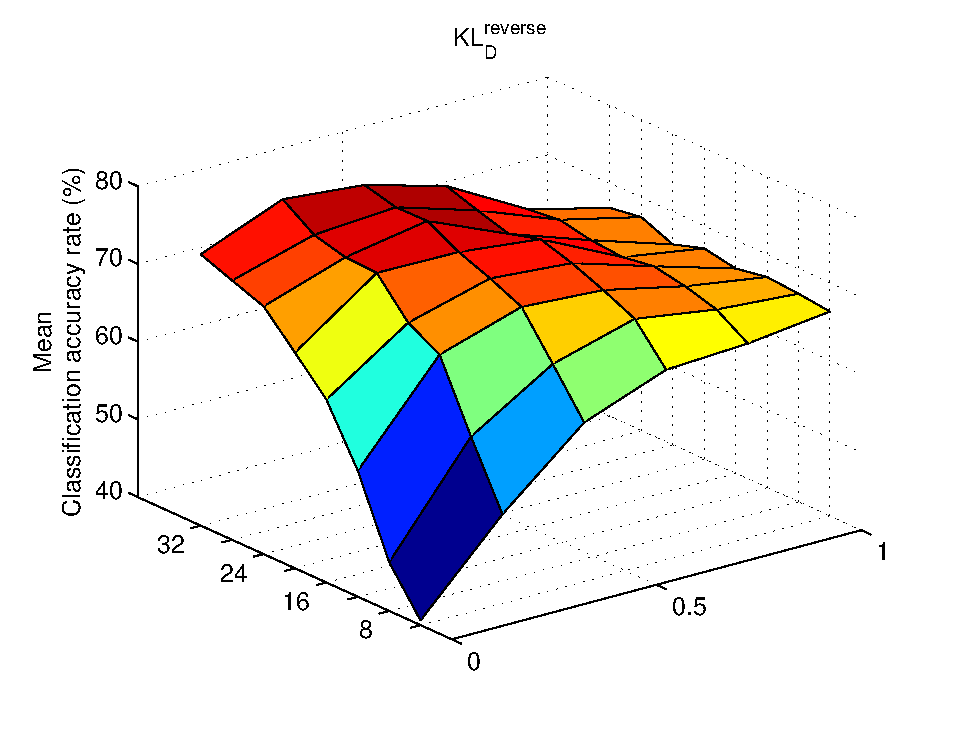
\includegraphics[width=0.47\textwidth]{Figures/surfmean_kld_rev.eps}
\label{fig:surfmean_kld_rev}}
\subfigure[]{
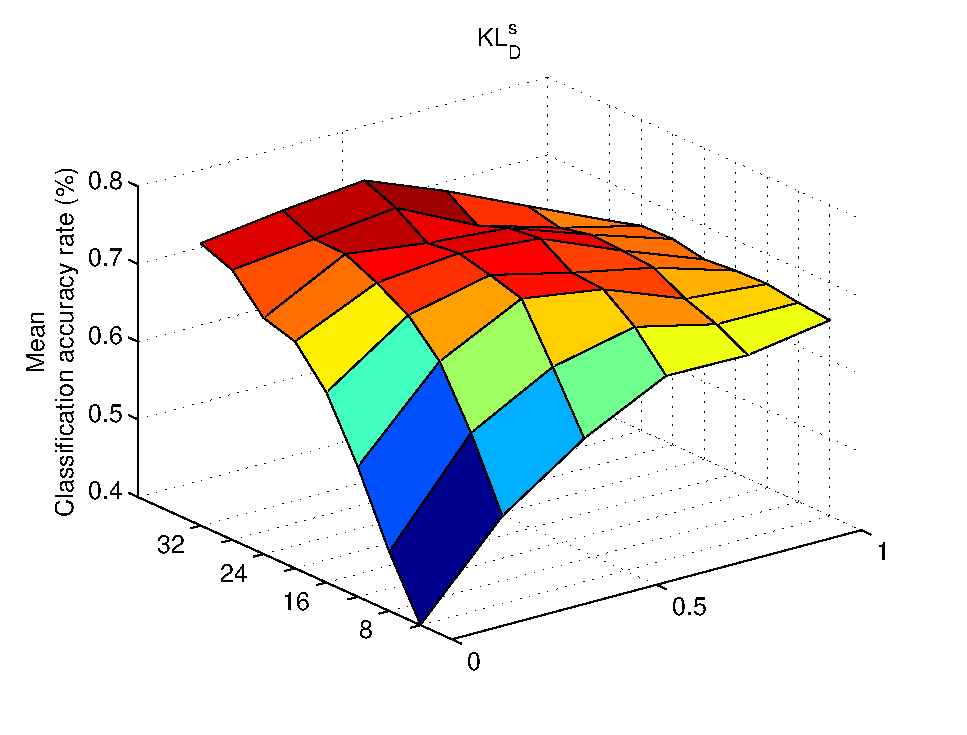
\includegraphics[width=0.47\textwidth]{Figures/surfmean_kld_sym.eps}
\label{fig:surfmean_kld_sym}}

\caption{Mean classification accuracy for 12 subjects. Grid search with different values of  $n \in \left\lbrace 4, 8, 12, 16, 20, 24, 28, 32 \right\rbrace $ on the x-axis and different values of $\lambda \in \left\lbrace 0, 0.2, 0.4, 0.6, 0.8, 1 \right\rbrace$ on the y-axis. The results are obtained using 4 metrics to measure similarity between subjects: \ref{fig:surfmean_airm} AIRM, \ref{fig:surfmean_kld_for} $\divB{KL}^{forward}$, \ref{fig:surfmean_kld_rev} $\divB{KL}^{reverse}$, \ref{fig:surfmean_kld_sym} $\divB{KL}^{symmetric}$}
\end{figure}

\begin{figure}[h!]
\centering
\subfigure[]{
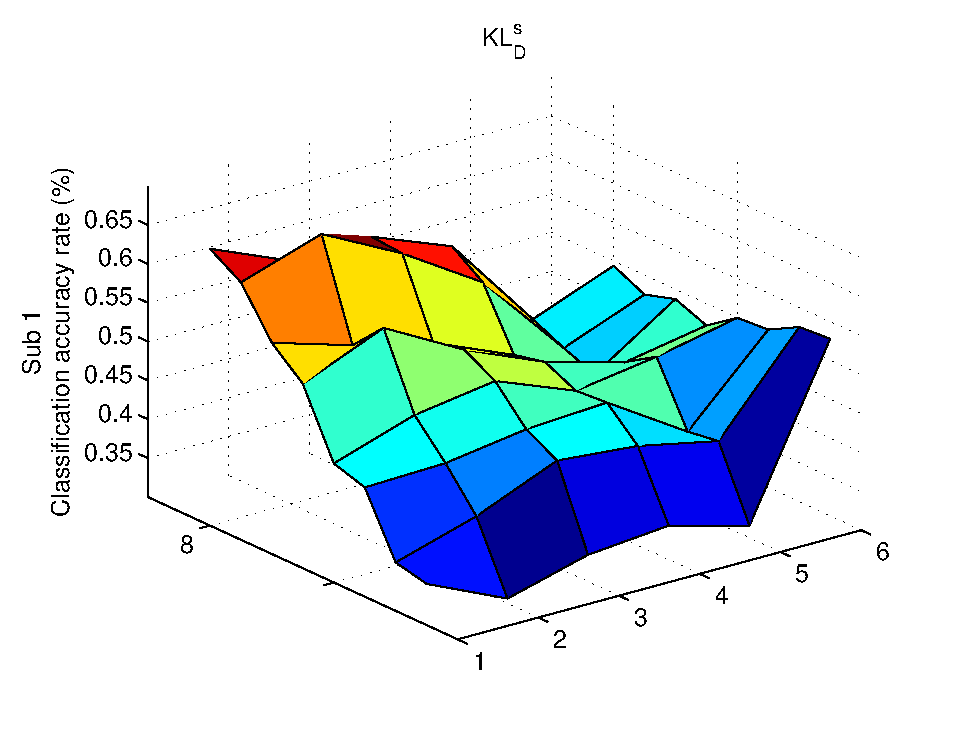
\includegraphics[width=0.3\textwidth]{Figures/surf_s1_kld_sym.eps}
\label{fig:surf_s1_kld_sym}}
\subfigure[]{
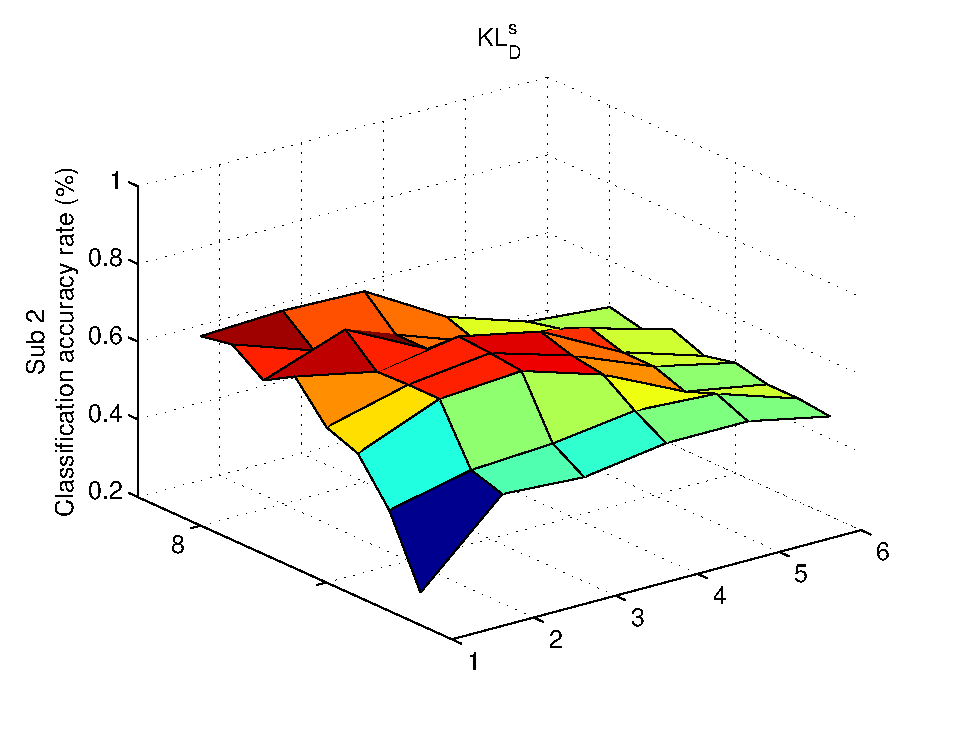
\includegraphics[width=0.3\textwidth]{Figures/surf_s2_kld_sym.eps}
\label{fig:surf_s2_kld_sym}}
\subfigure[]{
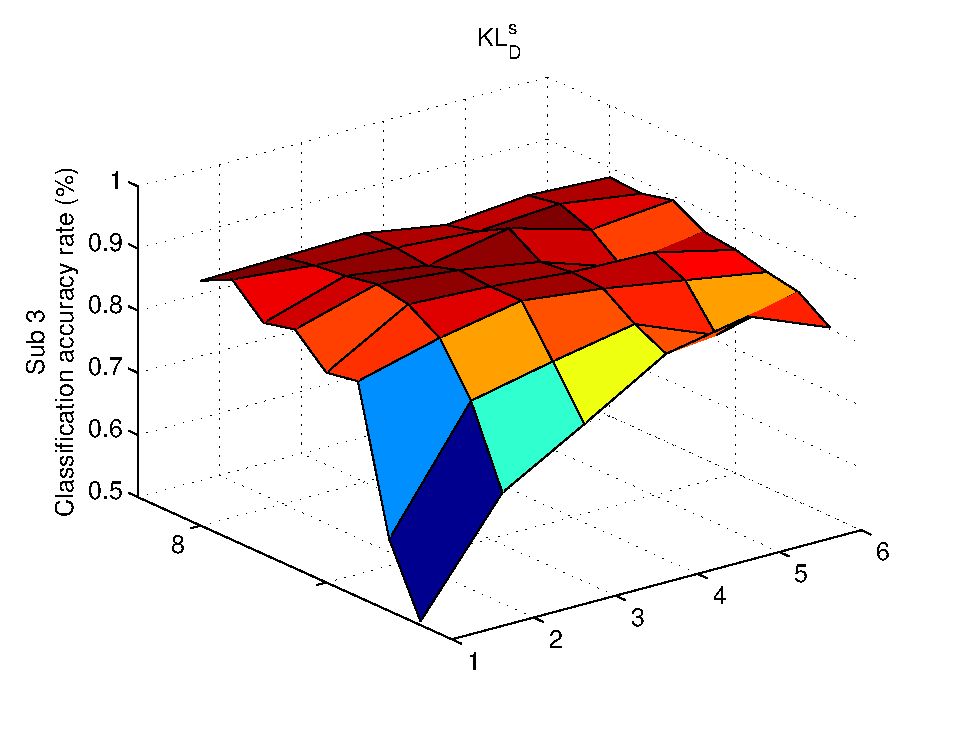
\includegraphics[width=0.3\textwidth]{Figures/surf_s3_kld_sym.eps}
\label{fig:surf_s3_kld_sym}}
\subfigure[]{
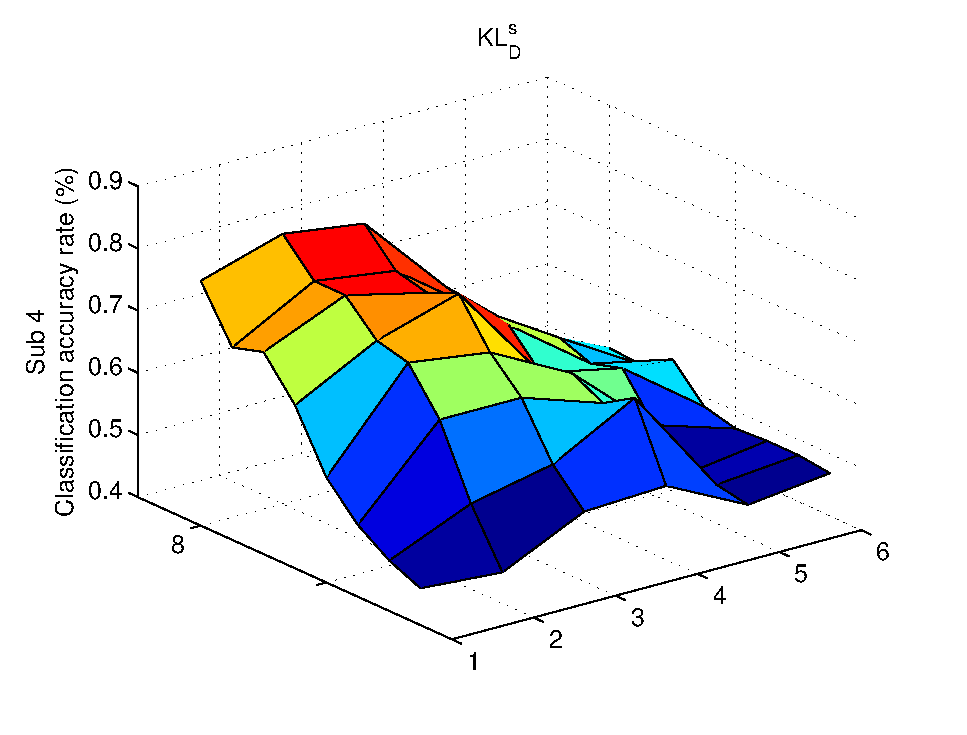
\includegraphics[width=0.3\textwidth]{Figures/surf_s4_kld_sym.eps}
\label{	}}
\subfigure[]{
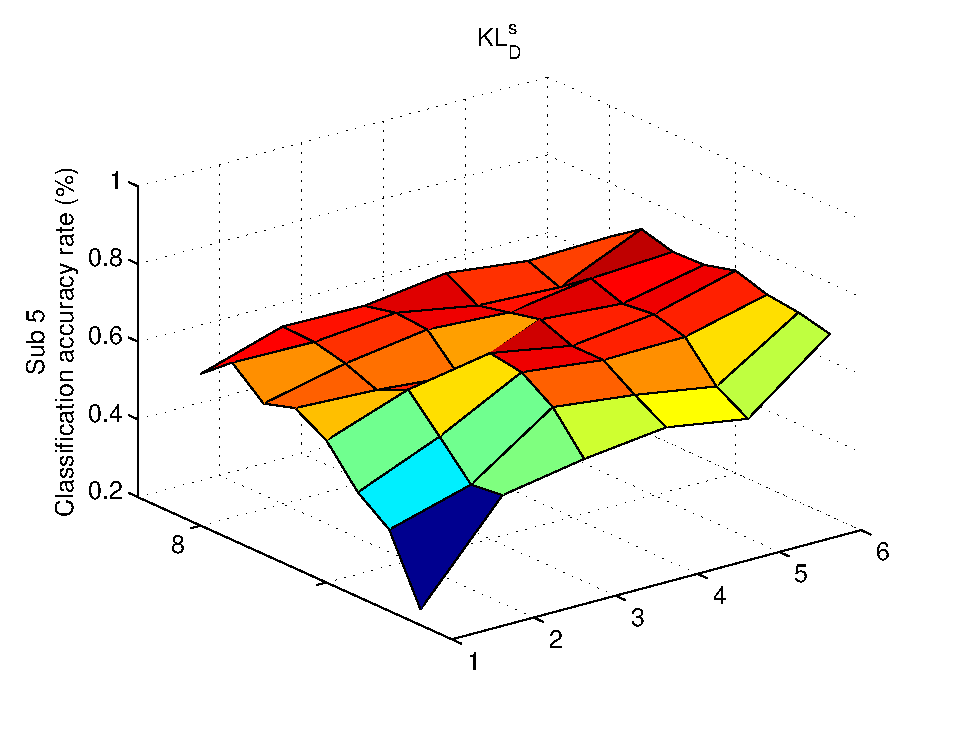
\includegraphics[width=0.3\textwidth]{Figures/surf_s5_kld_sym.eps}
\label{fig:surf_s5_kld_sym}}
\subfigure[]{
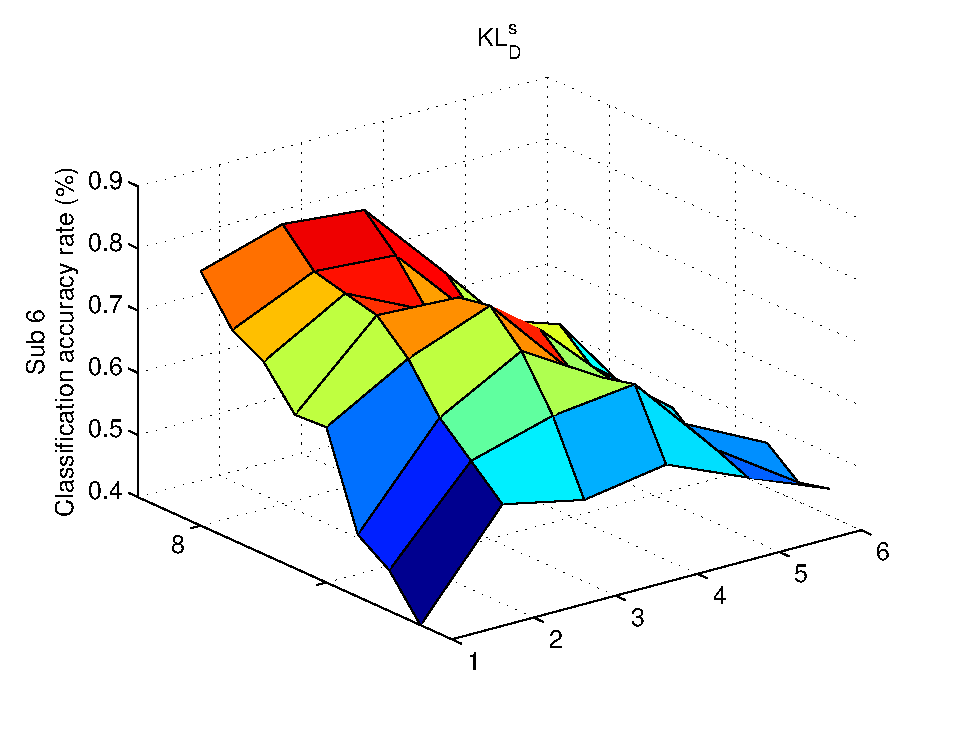
\includegraphics[width=0.3\textwidth]{Figures/surf_s6_kld_sym.eps}
\label{fig:surf_s6_kld_sym}}
\subfigure[]{
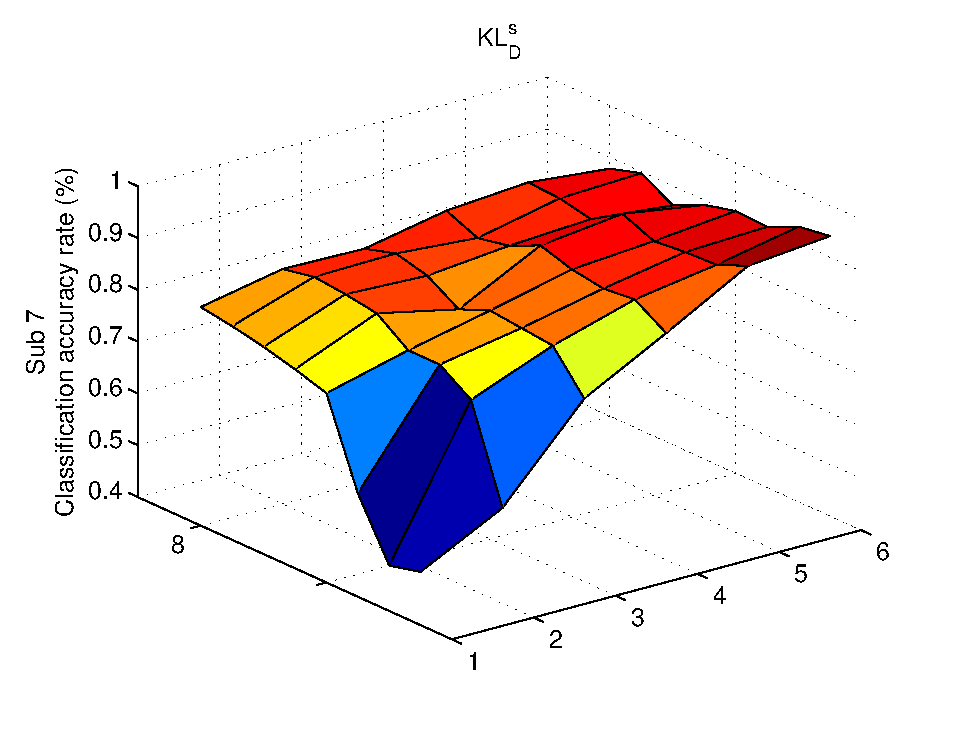
\includegraphics[width=0.3\textwidth]{Figures/surf_s7_kld_sym.eps}
\label{fig:surf_s7_kld_sym}}
\subfigure[]{
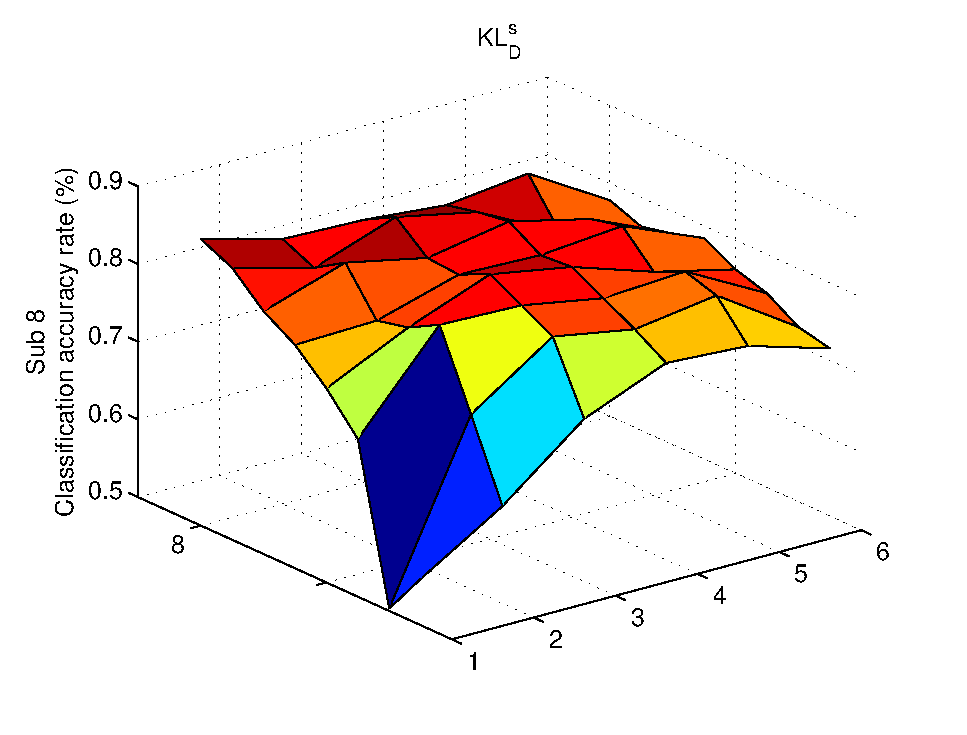
\includegraphics[width=0.3\textwidth]{Figures/surf_s8_kld_sym.eps}
\label{fig:surf_s8_kld_sym}}
\subfigure[]{
\includegraphics[width=0.3\textwidth]{Figures/surf_s9_kld_sym.eps}
\label{fig:surf_s9_kld_sym}}
\subfigure[]{
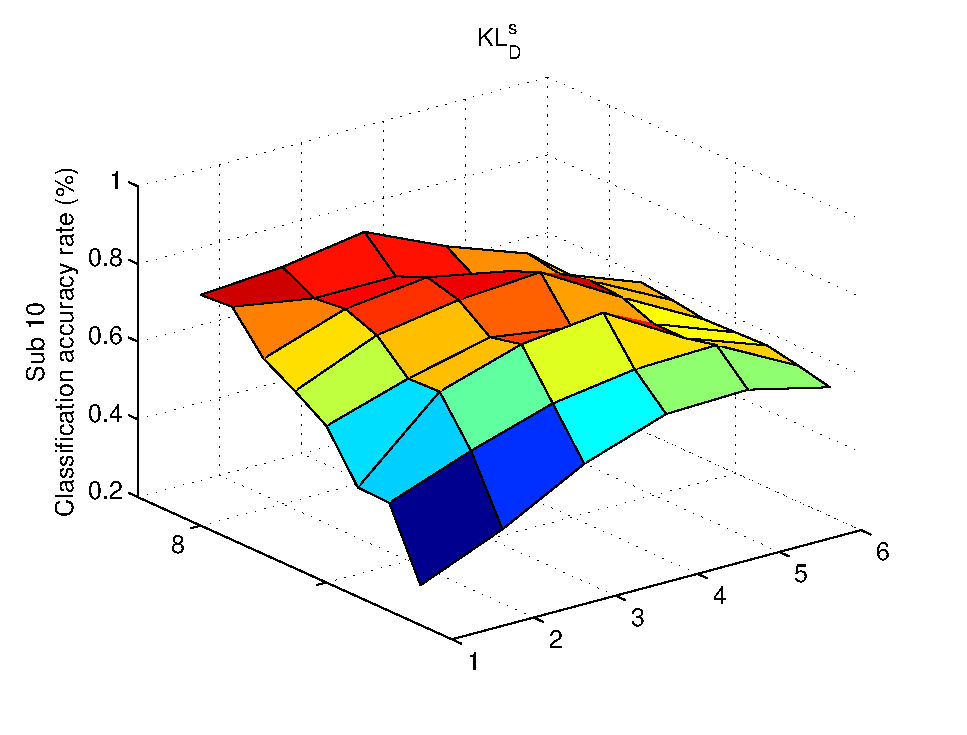
\includegraphics[width=0.3\textwidth]{Figures/surf_s10_kld_sym.eps}
\label{fig:surf_s10_kld_sym}}
\subfigure[]{
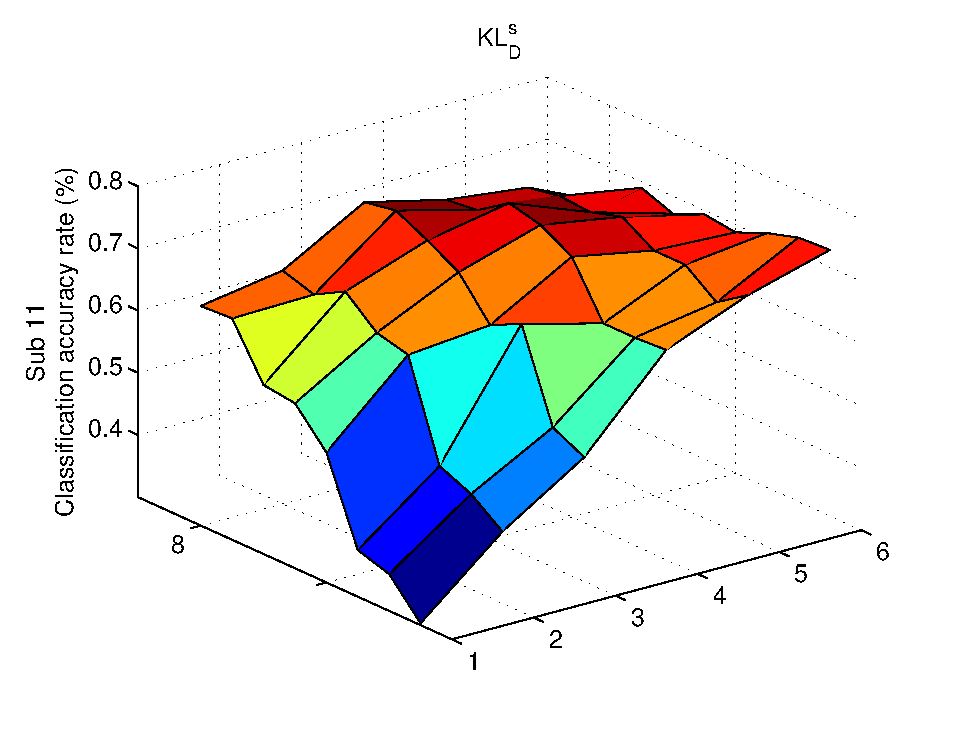
\includegraphics[width=0.3\textwidth]{Figures/surf_s11_kld_sym.eps}
\label{fig:surf_s11_kld_sym}}
\subfigure[]{
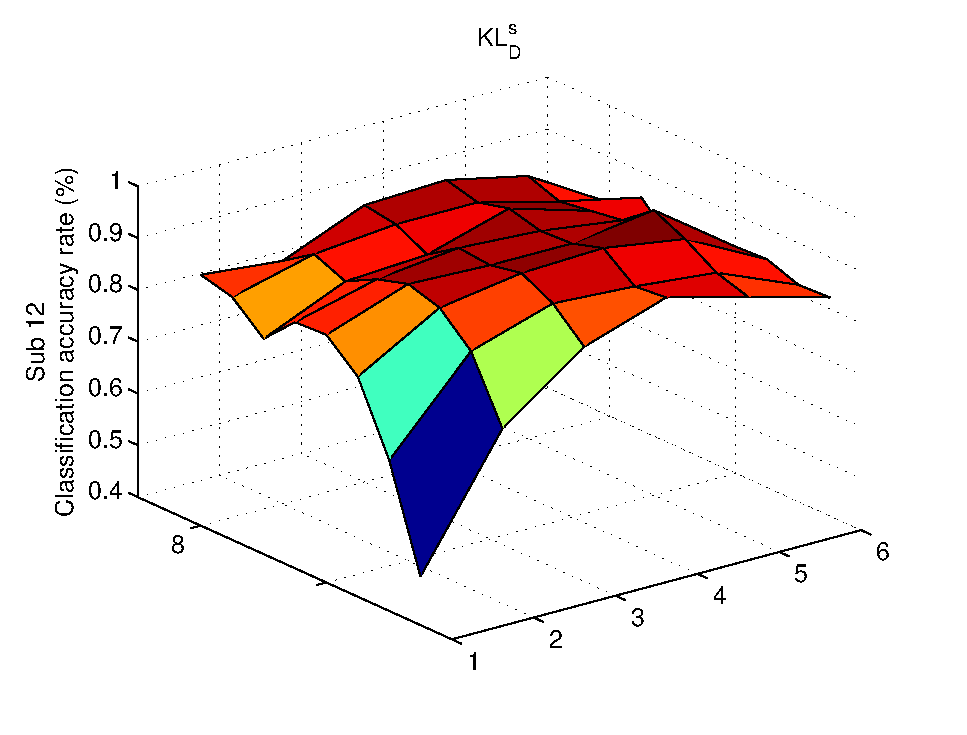
\includegraphics[width=0.3\textwidth]{Figures/surf_s12_kld_sym.eps}
\label{fig:surf_s12_kld_sym}}
\caption{Individual subject classification accuracy. Grid search with different values of  $n \in \left\lbrace 4, 8, 12, 16, 20, 24, 28, 32 \right\rbrace $ on the x-axis and different values of $\lambda \in \left\lbrace 0, 0.2, 0.4, 0.6, 0.8, 1 \right\rbrace$ on the y-axis. (a) to (l) correspond to subjects 1 to 12 respectively. The results are obtained using $\divB{KL}^{symmetric}$}
\end{figure}

\subsubsection{Evaluation $\lambda$}

Through the grid search, different values of $\lambda$ were tested with different numbers of samples. 
The optimal performances, i.e. the classification performance obtained with optimal $\lambda$, with each number available sample $n$ are compared with the performance obtained with $\lambda$ as defined in \eqref{eq:lambda}.
To this end a Pareto analysis is performed, with the Pareto front being the optimal classification accuracy obtained through a grid search.
Figure \ref{fig:pareto} shows the Pareto front against the performance obtained with $\lambda=1$, meaning only data from other subjects are considered for training, $\lambda=0$, only using test subjects' data, and $\lambda$ of \eqref{eq:lambda}.

\begin{figure}
\includegraphics[width=1\textwidth]{Figures/pareto}
\caption{Optimal performance (Pareto front) obtained through a grid search is compared with the performance with $\lambda = 0$, $\lambda = 1$, and $\lambda$ as proposed in \eqref{eq:lambda}.}
\label{fig:pareto}
\end{figure}

It is seen that the defined $\lambda$ performs well compared to the Pareto front. For $n > 4$, it even outperforms it. Indeed it allows for values between the intervals of those picked in the grid search. 

\section{Conclusion}
\label{sec:perspective-conclusion}

In BCI, cases of insufficient training data and/or unbalanced classes are frequent.
The section demonstrated that Riemannian geometry can be applied to address these issues through data augmentation and transfer learning.
A data augmentation scheme based on the geometry of covariance matrices was introduced.
From the geodesics passing through pairs of samples, new samples are drawn and fed to a neural classifier. 
The data augmentation allows to enhance the classification accuracy when there is only a few number of samples per class.
Data augmentation can compensate for dataset with unbalanced classes as it is often the case in event-related potential paradigm.
The choice of the classifier is important when dealing with this augmented data; neural networks yield the best results.
Future works will focus on the optimisation of the neural networks: determining the best architecture (in terms of layers and neurons) for processing covariance matrices and the investigation of common deep learning methods to improve results (dropouts, ReLU units, etc).
The perspective of transfer learning yield promising results. 
Further work should be done on the optimisation of parameters in the logistic function defining lambda through a cross validation process.
Other functions that could better describe the relationship between lambda, the proximity, and the number of training samples of the test subject should be explored.  

 
 

